% Options for packages loaded elsewhere
\PassOptionsToPackage{unicode}{hyperref}
\PassOptionsToPackage{hyphens}{url}
\PassOptionsToPackage{dvipsnames,svgnames,x11names}{xcolor}
%
\documentclass[
  letterpaper,
  DIV=11,
  numbers=noendperiod]{scrartcl}

\usepackage{amsmath,amssymb}
\usepackage{lmodern}
\usepackage{iftex}
\ifPDFTeX
  \usepackage[T1]{fontenc}
  \usepackage[utf8]{inputenc}
  \usepackage{textcomp} % provide euro and other symbols
\else % if luatex or xetex
  \usepackage{unicode-math}
  \defaultfontfeatures{Scale=MatchLowercase}
  \defaultfontfeatures[\rmfamily]{Ligatures=TeX,Scale=1}
\fi
% Use upquote if available, for straight quotes in verbatim environments
\IfFileExists{upquote.sty}{\usepackage{upquote}}{}
\IfFileExists{microtype.sty}{% use microtype if available
  \usepackage[]{microtype}
  \UseMicrotypeSet[protrusion]{basicmath} % disable protrusion for tt fonts
}{}
\makeatletter
\@ifundefined{KOMAClassName}{% if non-KOMA class
  \IfFileExists{parskip.sty}{%
    \usepackage{parskip}
  }{% else
    \setlength{\parindent}{0pt}
    \setlength{\parskip}{6pt plus 2pt minus 1pt}}
}{% if KOMA class
  \KOMAoptions{parskip=half}}
\makeatother
\usepackage{xcolor}
\setlength{\emergencystretch}{3em} % prevent overfull lines
\setcounter{secnumdepth}{-\maxdimen} % remove section numbering
% Make \paragraph and \subparagraph free-standing
\ifx\paragraph\undefined\else
  \let\oldparagraph\paragraph
  \renewcommand{\paragraph}[1]{\oldparagraph{#1}\mbox{}}
\fi
\ifx\subparagraph\undefined\else
  \let\oldsubparagraph\subparagraph
  \renewcommand{\subparagraph}[1]{\oldsubparagraph{#1}\mbox{}}
\fi


\providecommand{\tightlist}{%
  \setlength{\itemsep}{0pt}\setlength{\parskip}{0pt}}\usepackage{longtable,booktabs,array}
\usepackage{calc} % for calculating minipage widths
% Correct order of tables after \paragraph or \subparagraph
\usepackage{etoolbox}
\makeatletter
\patchcmd\longtable{\par}{\if@noskipsec\mbox{}\fi\par}{}{}
\makeatother
% Allow footnotes in longtable head/foot
\IfFileExists{footnotehyper.sty}{\usepackage{footnotehyper}}{\usepackage{footnote}}
\makesavenoteenv{longtable}
\usepackage{graphicx}
\makeatletter
\def\maxwidth{\ifdim\Gin@nat@width>\linewidth\linewidth\else\Gin@nat@width\fi}
\def\maxheight{\ifdim\Gin@nat@height>\textheight\textheight\else\Gin@nat@height\fi}
\makeatother
% Scale images if necessary, so that they will not overflow the page
% margins by default, and it is still possible to overwrite the defaults
% using explicit options in \includegraphics[width, height, ...]{}
\setkeys{Gin}{width=\maxwidth,height=\maxheight,keepaspectratio}
% Set default figure placement to htbp
\makeatletter
\def\fps@figure{htbp}
\makeatother

\usepackage{booktabs}
\usepackage{longtable}
\usepackage{array}
\usepackage{multirow}
\usepackage{wrapfig}
\usepackage{float}
\usepackage{colortbl}
\usepackage{pdflscape}
\usepackage{tabu}
\usepackage{threeparttable}
\usepackage{threeparttablex}
\usepackage[normalem]{ulem}
\usepackage{makecell}
\usepackage{xcolor}
\KOMAoption{captions}{tableheading}
\makeatletter
\makeatother
\makeatletter
\@ifpackageloaded{caption}{}{\usepackage{caption}}
\AtBeginDocument{%
\ifdefined\contentsname
  \renewcommand*\contentsname{Table of contents}
\else
  \newcommand\contentsname{Table of contents}
\fi
\ifdefined\listfigurename
  \renewcommand*\listfigurename{List of Figures}
\else
  \newcommand\listfigurename{List of Figures}
\fi
\ifdefined\listtablename
  \renewcommand*\listtablename{List of Tables}
\else
  \newcommand\listtablename{List of Tables}
\fi
\ifdefined\figurename
  \renewcommand*\figurename{Figure}
\else
  \newcommand\figurename{Figure}
\fi
\ifdefined\tablename
  \renewcommand*\tablename{Table}
\else
  \newcommand\tablename{Table}
\fi
}
\@ifpackageloaded{float}{}{\usepackage{float}}
\floatstyle{ruled}
\@ifundefined{c@chapter}{\newfloat{codelisting}{h}{lop}}{\newfloat{codelisting}{h}{lop}[chapter]}
\floatname{codelisting}{Listing}
\newcommand*\listoflistings{\listof{codelisting}{List of Listings}}
\makeatother
\makeatletter
\@ifpackageloaded{caption}{}{\usepackage{caption}}
\@ifpackageloaded{subcaption}{}{\usepackage{subcaption}}
\makeatother
\makeatletter
\@ifpackageloaded{tcolorbox}{}{\usepackage[many]{tcolorbox}}
\makeatother
\makeatletter
\@ifundefined{shadecolor}{\definecolor{shadecolor}{rgb}{.97, .97, .97}}
\makeatother
\makeatletter
\makeatother
\ifLuaTeX
  \usepackage{selnolig}  % disable illegal ligatures
\fi
\IfFileExists{bookmark.sty}{\usepackage{bookmark}}{\usepackage{hyperref}}
\IfFileExists{xurl.sty}{\usepackage{xurl}}{} % add URL line breaks if available
\urlstyle{same} % disable monospaced font for URLs
\hypersetup{
  pdftitle={Vizualizing Annual Energy Consumption in the GTA},
  pdfauthor={Sarah Mansoor},
  colorlinks=true,
  linkcolor={blue},
  filecolor={Maroon},
  citecolor={Blue},
  urlcolor={Blue},
  pdfcreator={LaTeX via pandoc}}

\title{Vizualizing Annual Energy Consumption in the GTA\thanks{Code and
data are available at:
https://github.com/sarahmansoorr/telling\_stories}}
\usepackage{etoolbox}
\makeatletter
\providecommand{\subtitle}[1]{% add subtitle to \maketitle
  \apptocmd{\@title}{\par {\large #1 \par}}{}{}
}
\makeatother
\subtitle{A Look Into How Energy Consumption has Changed from 2015 to
2018}
\author{Sarah Mansoor}
\date{21 June 2022}

\begin{document}
\maketitle
\begin{abstract}
Greenhouse gas emissions have a significant impact on the global climate
and are a key factor in climate change. This paper aims to examine the
greenhouse gas emissions in the GTA and their change between the years
2011 and 2018. I examine the data to find that there have has not been
much change in GHG emissions from 2015 to 2018 in the GTA.
\end{abstract}
\ifdefined\Shaded\renewenvironment{Shaded}{\begin{tcolorbox}[breakable, borderline west={3pt}{0pt}{shadecolor}, frame hidden, interior hidden, boxrule=0pt, sharp corners, enhanced]}{\end{tcolorbox}}\fi

\hypertarget{introduction}{%
\section{Introduction}\label{introduction}}

Climate change is one of the most significant environmental concerns of
our time. Climate change is caused by the development in concentrations
of greenhouse gases in the atmosphere. These increases are due to GHG
emissions using fossil fuels or agriculture. This changing climate has
effects on the environment, human health, and the economy.

Since 2015 and the signing of the Paris Agreement, Canada implemented
2005 as the base year for its GHG emission reduction target. In 2021,
Canada remained devoted to reduce its GHG emissions by 40 45 percent
below 2005 levels by 2030.

In most discussions around climate change, the focus tends to be on
carbon dioxide (CO2) which is the most dominant greenhouse gas that is
produced by the burning of fossil fuels. However, CO2 is not the only
greenhouse gas that drives climate change. Methane, nitrous oxcide, and
trace gases have contributed to a substantial amount of warming to
today. These greenhouse gases have different warming effects, for
example, one tonne of methane will not have the same impact on wamring
as one tonne of carbon dioxide.

I will explore GHG emissions in the GTA between the years 2015 and 2018
with respect to the operation type and the city. The dataset contains
annual energy consumption data for different cities around the GTA.
Through exploration of this data set, it can offer insights on ways to
reduce GHG emissions by further analyzing which operations produce the
most GHG emissions and which produces the least, as well as how these
emissions have changed from 2015 to 2018.

\pagebreak

\hypertarget{data}{%
\section{Data}\label{data}}

This assignment uses a data set from Open Data Toronto called Annual
Energy Consumption. This data set contains columns for the energy
consumption of individual buildings in Toronto that are required by
Ontario Regulation 397/11 and the Green Energy Act to report their GHG
emissions.

This data set contains 5561 observations with 6 variables with
information about energy consumption for different operations in
Toronto. This report will focus on operation name, operation type, city,
electricity quantity, GHG emissions (kg) and the year. The data set has
been cleaned for the 4 files from 2015 to 2018 using R and R packages:
``tidyverse'', ``dplyr'' and ``janitor''.

\hypertarget{visualizing-the-data-and-the-implications}{%
\section{Visualizing the Data and The
Implications}\label{visualizing-the-data-and-the-implications}}

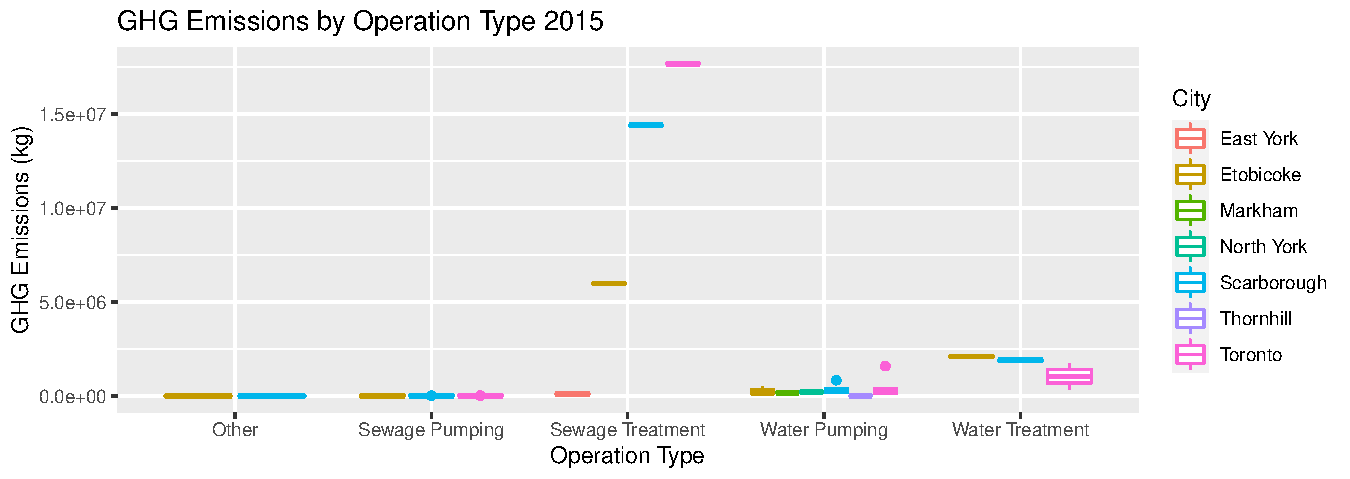
\includegraphics{paper_files/figure-pdf/unnamed-chunk-4-1.pdf}

\includegraphics{paper_files/figure-pdf/unnamed-chunk-4-2.pdf}

\includegraphics{paper_files/figure-pdf/unnamed-chunk-4-3.pdf}

\includegraphics{paper_files/figure-pdf/unnamed-chunk-4-4.pdf}

\includegraphics{paper_files/figure-pdf/unnamed-chunk-4-5.pdf}

\includegraphics{paper_files/figure-pdf/unnamed-chunk-4-6.pdf}

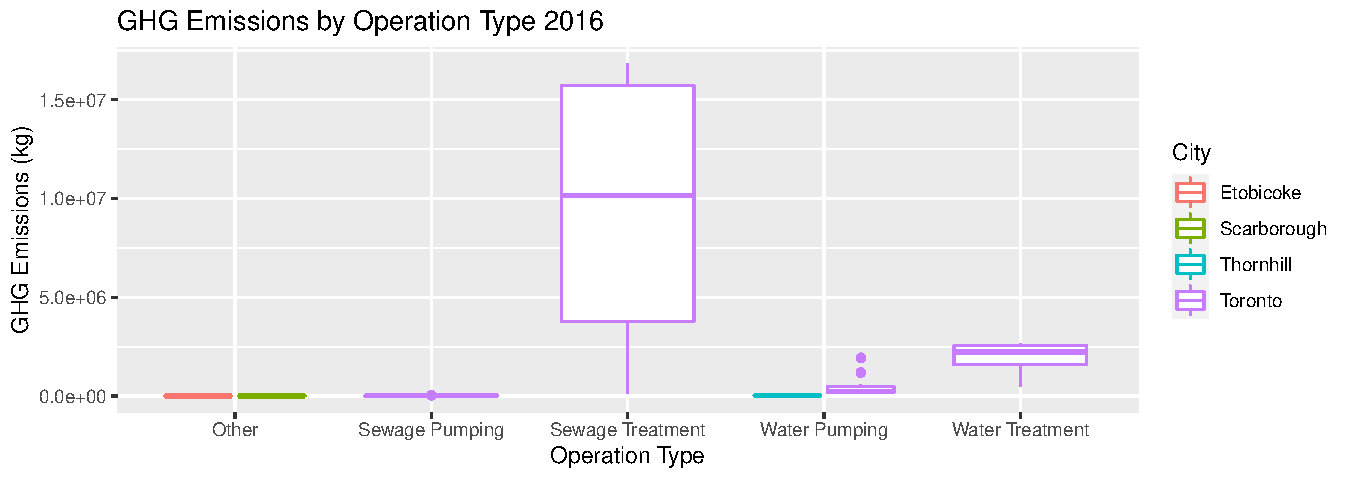
\includegraphics{paper_files/figure-pdf/unnamed-chunk-6-1.pdf}

\includegraphics{paper_files/figure-pdf/unnamed-chunk-6-2.pdf}

\includegraphics{paper_files/figure-pdf/unnamed-chunk-6-3.pdf}

\begin{table}[H]

\caption{Extracting rows from the Annual Energy Consumption Data}
\centering
\fontsize{10}{12}\selectfont
\begin{tabular}[t]{llrr}
\toprule
Operation Type & City & GHG Emissions (kg) & Year\\
\midrule
Parking garages & Toronto & 23452.67 & 2015\\
Water Pumping & Toronto & 2225.77 & 2015\\
Police Station & Toronto & 158824.69 & 2016\\
Police Station & Toronto & 204678.78 & 2016\\
Administrative Offices & Toronto & 46579.55 & 2017\\
Ambulance Station & North York & 635149.57 & 2017\\
Administrative Offices & Etobicoke & 103471.39 & 2018\\
Ambulance Station & Etobicoke & 1665.87 & 2018\\
Water Treatment & Toronto & 1918035.82 & 2018\\
\bottomrule
\end{tabular}
\end{table}

\hypertarget{next-steps}{%
\section{Next Steps}\label{next-steps}}

After analyzing this data set, it can be observed that the GHG emissions
are still very high throughout the GTA and there should be efforts to
reduce these emissions. There should be further analysis done on the
sewage and water treatment operations to find out what has been causing
the high GHG emissions for these operations.



\end{document}
